\chapter{When transitions are uniform POIBMDPs are fully observable}
In this section we show that decision tree induction for classification problems can be formulated as solving POIBMDPs.
Indeed, a classification problem can be formulated as an MDP where actions are class labels and states are training data.
The reward at every step is 1 if the correct label was predicted and 0 otherwise.
In this MDP, the transitions are independent of the actions: the next state is given by uniformly sampling a new training datum. 
This implies that the resulting POIBMDP is actually \textit{fully} observable and that traditional RL algorithms should perform well.

After showing the equivalence between decision tree induction and solutions to POIBMDPs when the underlying base MDP encodes a classification task, we call them Classification-POIBMDPs, we highlight key limitations of the RL approach for decision tree induction.
There are few other RL approaches for decision tree induction (cite). Here we focus on RL for Classification-POIBMDPs
We defer the formal definition of classification tasks in the supervised learning setting in the next chapter and rather directly define an MDP that encodes such tasks. 
\begin{definition}[Classification Markov Decision Process]
    Given a set of $N$ examples denoted $\mathcal{E} = {\{(x_i, y_i)\}}_{i=1}^N$ where each datum $x_i$ is described by a set of $p$ features and $y_i \in \mathbb{Z}^m$ is the label associated with $x_i$, a Classification Markov Decision Process is an MDP (cite) $\langle S, A, R, T, T_0 \rangle$ where:
    \begin{itemize}
        \item the state space is $S={\{x_i\}}_{i=1}^N$, the set of data features
        \item the action space is $A=\mathbb{Z}^m$, the set of unique labels
        \item the reward function is $R:S\times A \rightarrow \{0, 1\}$ with $R(s=x_i, a) = 1_{a=y_i}$
        \item the transition function is $T:S\times A \rightarrow \Delta S$ with $T(s, a, s') = \frac{1}{N} \quad \forall s, a, s'$
        \item the initial distribution is $T_0(s_0 = s) = \frac{1}{N}$
    \end{itemize}
\end{definition}
It is easy to see that policies that maximize the expected dsicounted cumulative reward objective (cite) are classifiers that maximize the prediction accuracy $\sum_{i=1}^N 1_{\pi(x_i)=y_i} = \sum_{i=1}^N R(x_i, \pi(x_i))$.
Learning a classifier with a reward signal can also be done with contextual bandits (cite).

To learn a decision tree classifier, we use the POIBMDP formalism and show in the particular case of the base MDP being a Classification MDP, the POIBMDP is in fact an MDP with stochastic transitions. 

\begin{definition}[Classification POIBMDP]
    Given a classification MDP (cite) $\langle {\{x_i\}}_{i=1}^N, \mathbb{Z}^m, R, T, T_0 \rangle$, and an associated POIBMDP (cite) $\langle S, O, A, A_{info}, R, \zeta, T_{info}, T, T_0\rangle$, a classification POIBMDP is an MDP:
    \begin{align*}
        \langle \overbrace{O}^{\text{State space}}, \underbrace{\mathbb{Z}^m, A_{info}}_{\text{Action space}}, \overbrace{R, \zeta}^{\text{Reward function}}, \underbrace{\mathcal{P}, \mathcal{P}_0}_{\text{Transition kernels}} \rangle
    \end{align*}
    \begin{itemize}
        \item $O$ is the set of possible observations in $[L_1, U_1] \times \dots \times [L_d, U_d] \times [L_1, U_1] \ times \dots \times [L_d, U_d] $ where $L_j$ is the minimum value of feature $j$ over all data $x_i$ and $U_j$ the maximum
        \item $\mathbb{Z}^m \cup A_{info}$ is action space: actions can be label assignments in $\mathbb{Z}^m$ or bounds refinement in $A_{info}$
        \item The reward for assigning label $a\in \mathbb{Z}^m$ when observing some observation $o=(L'_1, U'_1, \dots, L'_d, U'_d)$ is the proportion of training data satistifying the bounds and having label $a$: $R(o, a) = \frac{|\{x_i: L'_j \leq x_{ij} \leq U'_j \forall i,j \} \cap \{x_i: y_i = a \forall i \}|}{|\{x_i: L'_j \leq x_{ij} \leq U'_j \forall i,j \}|}$. 
        The reward for taking an information gathering action that refines bounds is $\zeta$
        \item The transition kernel is $\mathcal{P}:O \times (\mathbb{Z}^m \cup A_{info}) \rightarrow \Delta O$ where:
        \begin{itemize}
            \item For $a \in \mathbb{Z}^m$: $\mathcal{P}(o, a, (L_1, U_1, \dots, L_d, U_d)) = 1$ (reset to full bounds)
            \item For $a = (k, v) \in A_{info}$: from $o=(L'_1, U'_1, \dots, L'_d, U'_d)$, the MDP will transit to $o_{left} = (L'_1, U'_1, \dots, L_k, v, dots, L'_d, U'_d)$ (resp. $o_{right} = (L'_1, U'_1, \dots, U'_k, v, dots, L'_d, U'_d)$) with probability $\frac{|\{x_i: L'_j \leq x_{ij} \leq U'_j \forall j \land x_{ik} \leq v\}|}{|\{x_i: L'_j \leq x_{ij} \leq U'_j \forall j\}|}$ (resp. $\frac{|\{x_i: L'_j \leq x_{ij} \leq U'_j \forall j \land x_{ik} > v\}|}{|\{x_i: L'_j \leq x_{ij} \leq U'_j \forall j\}|}$)
        \end{itemize}
    \end{itemize}
\end{definition}
\begin{figure}
    \centering
    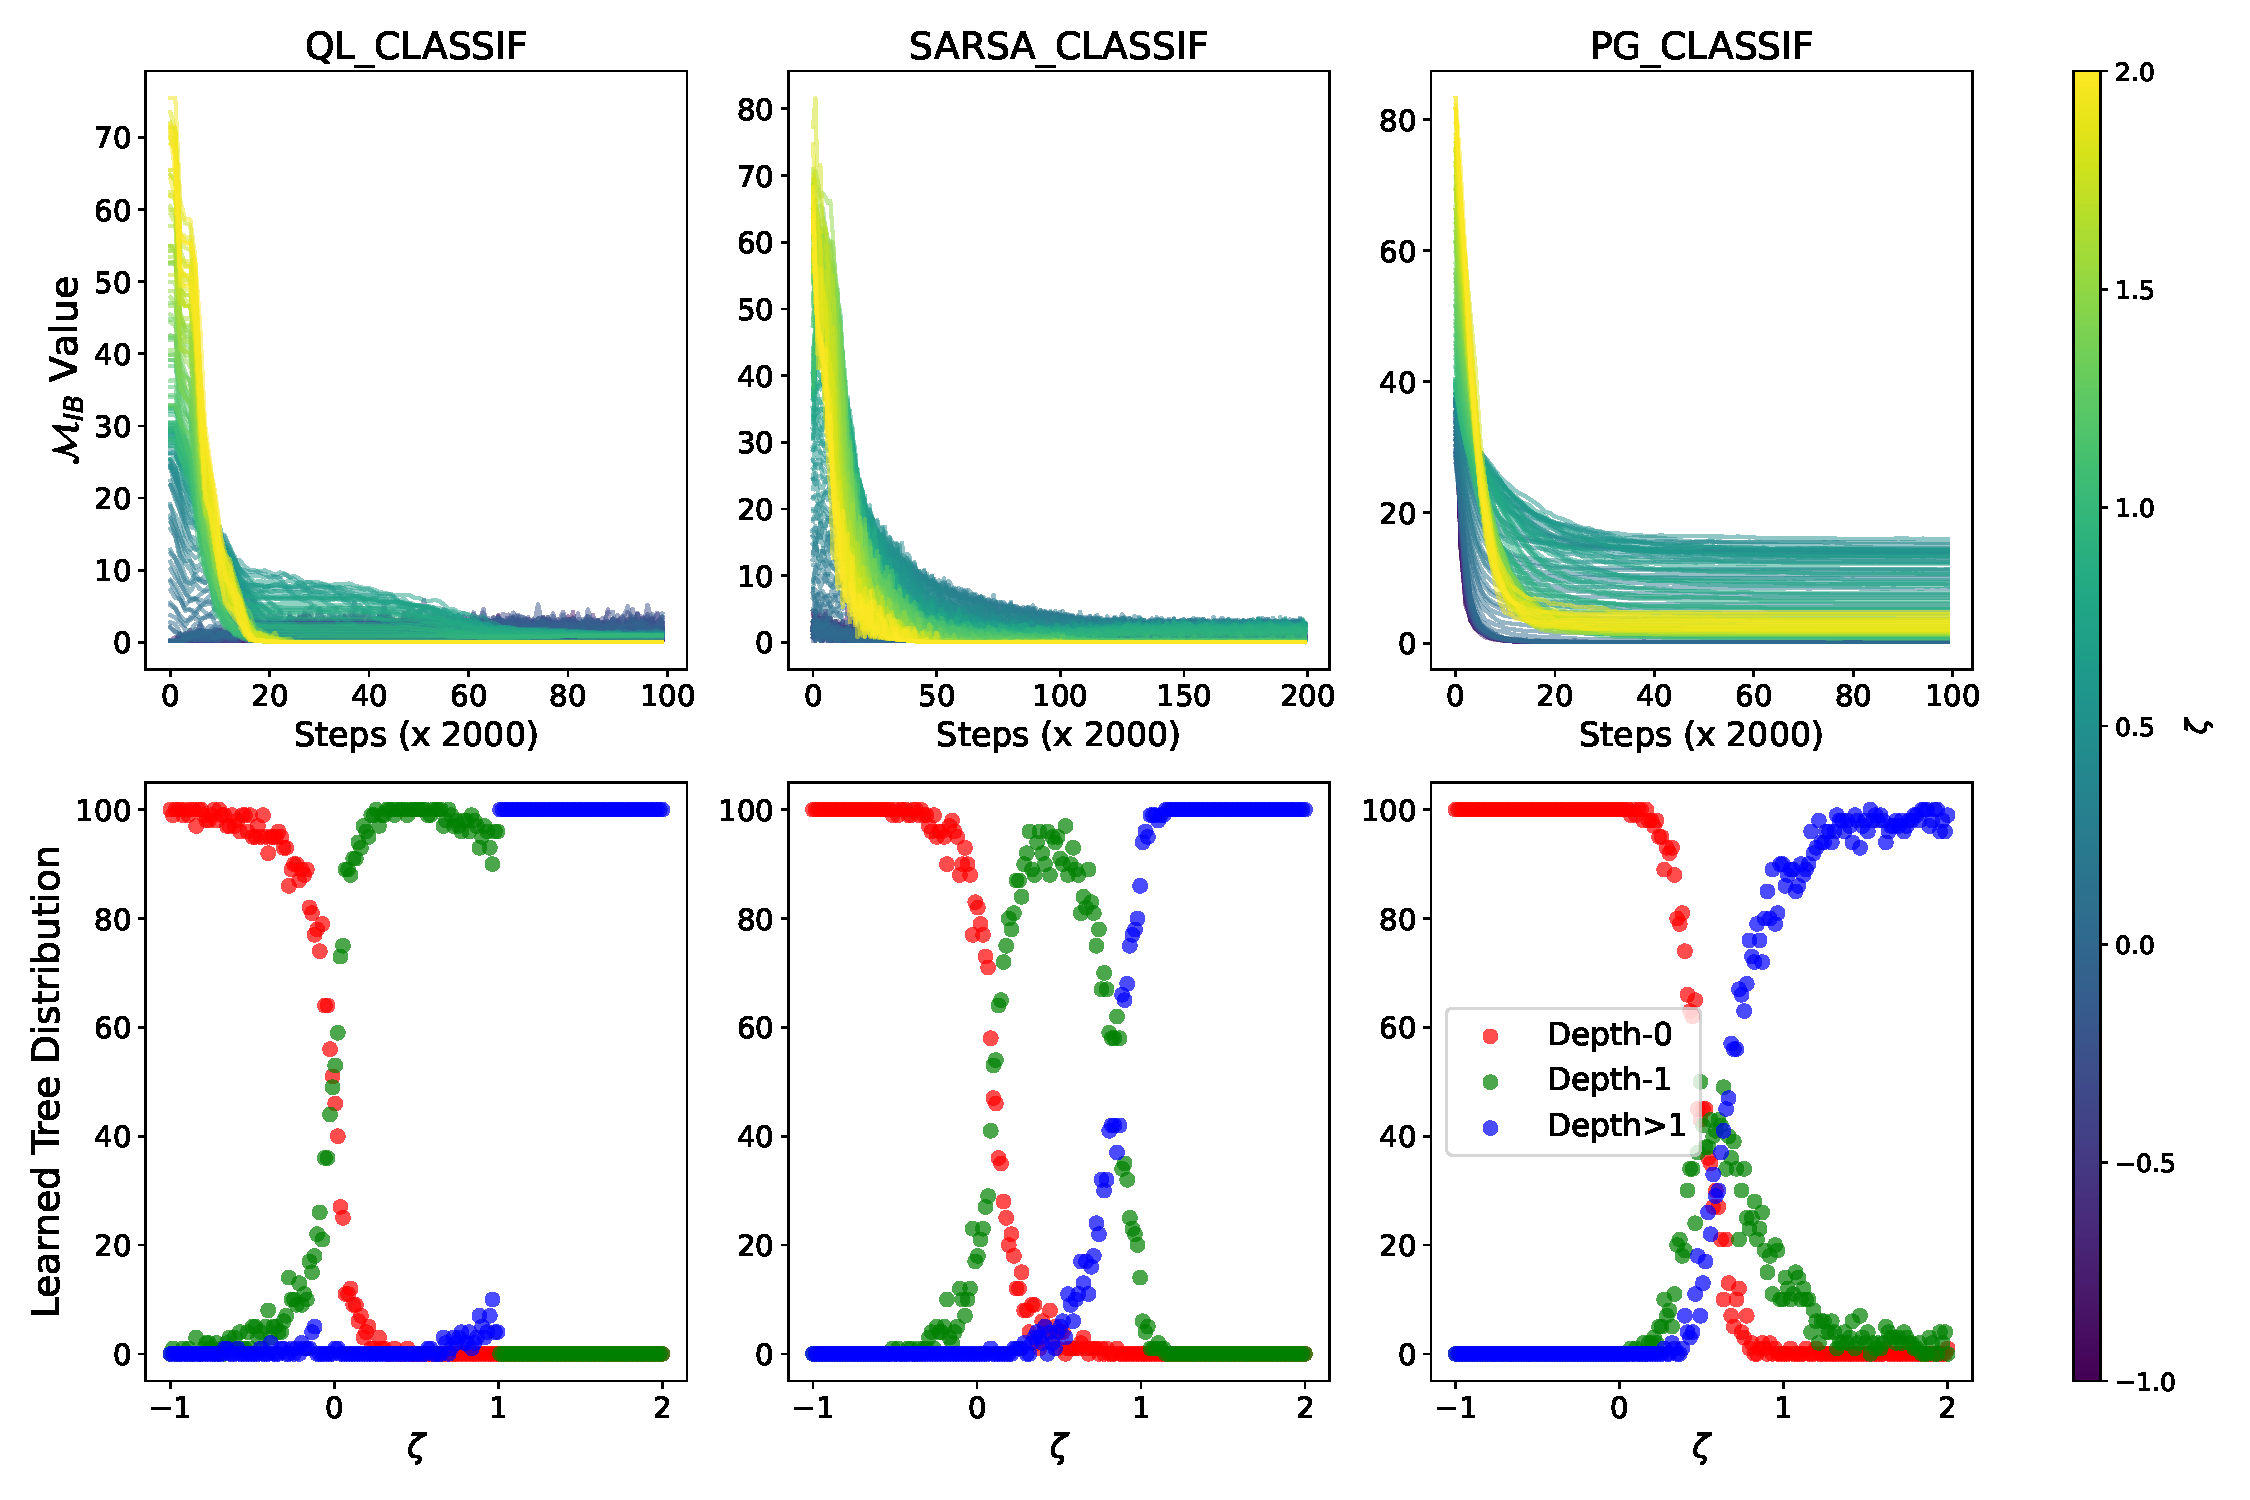
\includegraphics[width=1\textwidth]{images/images_part1/quick_plot_combined_classif.pdf}
    \caption{RL algorithms for classification OIBMDPs}\label{fig:rl-classif-poibmdp}
\end{figure}
